\documentclass[aspectratio=169]{../latex_main/tntbeamer}  % you can pass all options of the beamer class, e.g., 'handout' or 'aspectratio=43'
\usepackage{dsfont}
\usepackage{bm}
\usepackage[english]{babel}
\usepackage[T1]{fontenc}
%\usepackage[utf8]{inputenc}
\usepackage{graphicx}
\graphicspath{ {./figures/} }
\usepackage{algorithm}
\usepackage[ruled,vlined,algo2e,linesnumbered]{algorithm2e}
\usepackage{hyperref}
\usepackage{booktabs}
\usepackage{mathtools}

\usepackage{amsmath,amssymb}

\DeclareMathOperator*{\argmax}{arg\,max}
\DeclareMathOperator*{\argmin}{arg\,min}

\usepackage{amsbsy}
\newcommand{\vect}[1]{\bm{#1}}
%\newcommand{\vect}[1]{\boldsymbol{#1}}

\usepackage{pgfplots}
\pgfplotsset{compat=1.16}
\usepackage{tikz}
\usetikzlibrary{trees} 
\usetikzlibrary{shapes.geometric}
\usetikzlibrary{positioning,shapes,shadows,arrows,calc,mindmap}
\usetikzlibrary{positioning,fadings,through}
\usetikzlibrary{decorations.pathreplacing}
\usetikzlibrary{intersections}
\pgfdeclarelayer{background}
\pgfdeclarelayer{foreground}
\pgfsetlayers{background,main,foreground}
\tikzstyle{activity}=[rectangle, draw=black, rounded corners, text centered, text width=8em]
\tikzstyle{data}=[rectangle, draw=black, text centered, text width=8em]
\tikzstyle{myarrow}=[->, thick, draw=black]

% Define the layers to draw the diagram
\pgfdeclarelayer{background}
\pgfdeclarelayer{foreground}
\pgfsetlayers{background,main,foreground}

% Requires XeLaTeX or LuaLaTeX
%\usepackage{unicode-math}

\usepackage{fontspec}
%\setsansfont{Arial}
\setsansfont{RotisSansSerifStd}[ 
Path=../latex_main/fonts/,
Extension = .otf,
UprightFont = *-Regular,  % or *-Light
BoldFont = *-ExtraBold,  % or *-Bold
ItalicFont = *-Italic
]
\setmonofont{Cascadia Mono}[
Scale=0.8
]

% scale factor adapted; mathrm font added (Benjamin Spitschan @TNT, 2021-06-01)
%\setmathfont[Scale=1.05]{Libertinus Math}
%\setmathrm[Scale=1.05]{Libertinus Math}

% other available math fonts are (not exhaustive)
% Latin Modern Math
% XITS Math
% Libertinus Math
% Asana Math
% Fira Math
% TeX Gyre Pagella Math
% TeX Gyre Bonum Math
% TeX Gyre Schola Math
% TeX Gyre Termes Math

% Literature References
\newcommand{\lit}[2]{\href{#2}{\footnotesize\color{black!60}[#1]}}

%%% Beamer Customization
%----------------------------------------------------------------------
% (Don't) Show sections in frame header. Options: 'sections', 'sections light', empty
\setbeamertemplate{headline}{empty}

% Add header logo for normal frames
\setheaderimage{
	% 
\includegraphics[height=\logoheight]{figures/TNT_darkv4.pdf}
	
\includegraphics[height=\logoheight]{../latex_main/figures/luh_logo_rgb_0_80_155.pdf}
	% 
\includegraphics[height=\logoheight]{figures/logo_tntluh.pdf}
}

% Header logo for title page
\settitleheaderimage{
	% 
\includegraphics[height=\logoheight]{figures/TNT_darkv4.pdf}
	
\includegraphics[height=\logoheight]{../latex_main/figures/luh_logo_rgb_0_80_155.pdf}
	% 
\includegraphics[height=\logoheight]{figures/logo_tntluh.pdf}
}

% Title page: tntdefault 
\setbeamertemplate{title page}[tntdefault]  % or luhstyle
% Add optional title image here
%\addtitlepageimagedefault{
\includegraphics[width=0.65\textwidth]{figures/luh_default_presentation_title_image.jpg}}

% Title page: luhstyle
% \setbeamertemplate{title page}[luhstyle]
% % Add optional title image here
% \addtitlepageimage{
\includegraphics[width=0.75\textwidth]{figures/luh_default_presentation_title_image.jpg}}

\author[Abedjan \& Lindauer]{Ziawasch Abedjan \& Marius Lindauer\\[1em]
	
\includegraphics[height=\logoheight]{../latex_main/figures/luh_logo_rgb_0_80_155.pdf}\qquad
	
\includegraphics[height=\logoheight]{../latex_main/figures/DBIS_Kurzlogo.png}\qquad

\includegraphics[height=\logoheight]{../latex_main/figures/TNT_darkv4}\qquad

\includegraphics[height=\logoheight]{../latex_main/figures/L3S.jpg}	}
\date{Summer Term 2022; \hspace{0.5em} {
\includegraphics[height=1.5em]{../latex_main/figures/Cc-by-nc-sa_icon.svg.png}}; based on \href{https://ds100.org/fa21/}{[DS100]}
}


%%% Custom Packages
%----------------------------------------------------------------------
% Create dummy content
\usepackage{blindtext}

% Adds a frame with the current page layout. Just call \layout inside of a frame.
\usepackage{layout}


%%% Macros
%\renewcommand{\vec}[1]{\mathbf{#1}}
% \usepackage{bm}
%\let\vecb\bm

\title[Introduction]{DS: Introduction to Modeling}
\subtitle{Loss functions}

\graphicspath{ {./figure/} }
%\institute{}


\begin{document}
	
	\maketitle
	\begin{frame}{The cost of doing business (making predictions)}
	    We need some metric of how “good” or “bad” our predictions are. This is what loss functions provide us with. Loss functions quantify how bad a prediction is for a single observation.
	    \begin{itemize}
	        \item If our prediction is close to the actual value, we want low loss.
	        \item If our prediction is far from the actual value, we want high loss.
	    \end{itemize}
	    \bigskip
	    A natural choice of loss function is actual - predicted, or      $y_i - \hat{y_i}$.  We call this the error for a single prediction.
	    \begin{itemize}
	        \item But, this treats “negative” predictions and “positive” predictions differently. 
	        \begin{itemize}
	            \item Predicting 16 when the true value is 15 should be penalized the same as predicting 14.
	        \end{itemize}
	        \item This leads to two natural loss functions. 
	    \end{itemize}
	    
	\end{frame}
	
	
	\begin{frame}{Squared and absolute loss}
	    The most common loss function you’ll see is the squared loss, also known as L2 loss.\\
	       \hspace{5cm} $L_2(y,\hat{y})  = (y-\hat{y})^2$
            \bigskip
	    \begin{itemize}
	        \item For a single data point in general, this is          $(y_i- \hat{y}_i)^2$.
	        \item For our constant model, since    $\hat{y} = \theta$, this is     $(y_i - \theta)^2$.
	    \end{itemize}
	    \bigskip
	    Another common loss function is the absolute loss, also known as L1 loss.\\
	       \hspace{5cm} $L_1(y, \hat{y}) = |y-\hat{y}|$
            \bigskip
	    \begin{itemize}
	        \item For our constant model, for a single point, this is      $|y_i - \theta|$.
	    \end{itemize}
	    There are benefits and drawbacks to both of the above loss functions. We will examine those shortly. These are also not the only possible loss functions; we will see more later.
	    
	    \vspace{-5cm}
	    \hspace{10cm}  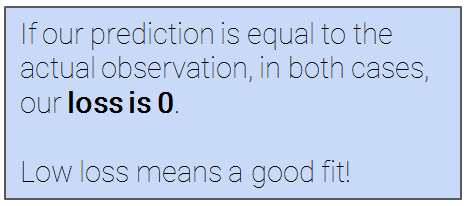
\includegraphics[scale=.35]{Bild21}
	\end{frame}
	
	
	\begin{frame}{Loss functions and empirical risk}
	    We care about how bad our model’s predictions are for our entire data set, not just for one point. A natural measure, then, is of the average loss across all points.  Assuming   n   points:\\
	    \begin{equation*}
	        \frac{1}{n}\sum\limits_{i=1}^nL(y_i, \hat{y}_i)
	    \end{equation*}
	    
	    \bigskip
	    The average loss of a model tells us how well it fits the given data. If our model has a low average loss across our dataset, that means it is good at making predictions. As such, we want to find the parameter(s) that minimize average loss, in order to make our model as good at making predictions as it can be.\\
	    
        \vspace{-3.5cm}
        \hspace{8.5cm}
        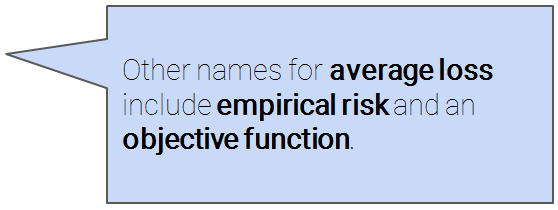
\includegraphics[scale=.3]{Bild22}
	    
	\end{frame}
	
	
	\begin{frame}{MSE and MAE}
	    If we choose squared loss as our loss function, then average squared loss is typically referred to as mean squared error (MSE), and is of the following form: 
	    \begin{equation*}
	        MSE(y, \hat{y}) = \frac{1}{n}\sum\limits_{i=1}^n(y_i - \hat{y}_i)^2
	    \end{equation*}
	    \bigskip\\
	    If we choose absolute loss as our loss function, then average absolute loss is typically referred to as mean absolute error (MAE), and is of the following form:
	    \begin{equation*}
	        MAE(y, \hat{y}) = \frac{1}{n}\sum\limits_{i=1}^n|y_i - \hat{y}_i|
	    \end{equation*}
	    These definitions hold true, regardless of our model. We want to minimize these quantities.
	   
	\end{frame}
	
	\begin{frame}{Exploring MSE}
	    Average loss is typically written as a function of  $\theta$  , since  $\theta$   defines what our model is (and hence what our predictions are). For example, with squared loss and the constant model, our average loss (and hence, the function we want to minimize) is\\
	  
	    \hspace{5cm} $R(\theta) = \frac{1}{n}\sum\limits_{i=1}^n(y_i - \theta)^2$\\
	    \vspace{-1.3cm}
	    \hspace{10cm} 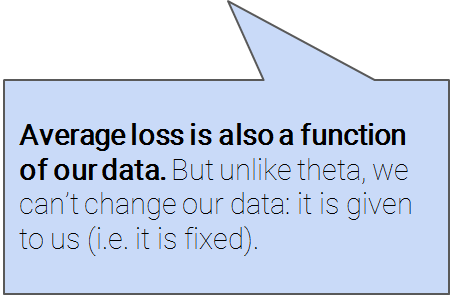
\includegraphics[scale=.3]{Bild23}\\
	    %\vspace{8cm}
	    
	     Mathematically, our goal of finding the optimal   $\hat{\theta}$  is stated as:\\
	    \vspace{.5cm}
	    \hspace{.3cm}
	    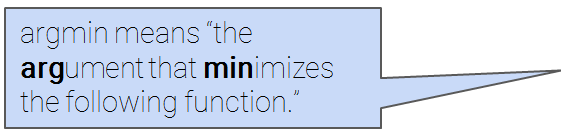
\includegraphics[scale=.35]{Bild24}\\
	    
	    \vspace{-1.3cm}
	    \hspace{4.5cm} $\hat{\theta} = \underset{\theta}{\text{arg min}} \frac{1}{n}\sum\limits_{i=1}^n(y_i - \theta)^2$\\
	    \vspace{0.5cm}
	    We won’t use this notation again in this lecture, but it will come up again in the future.\\
	\end{frame}
	
	
	
	\begin{frame}{Exploring MSE}
	    When our model is the constant model, and we choose to use L2 loss, again, our average loss looks like:
	    \begin{equation*}
	        R(\theta) = \frac{1}{n}\sum\limits_{i=1}^n(y_i - \theta)^2
	    \end{equation*}
	    Let’s examine a toy example. Suppose we have 5 observations, [20, 21, 22, 29, 33].
	    \begin{equation*}
	        L_2(20,\theta) = (20 - \theta)^2 \hspace{1cm} R(\theta) = \frac{1}{5}((20 - \theta)^2 + (21-\theta)^2 + (22 - \theta)^2 + (29 - \theta)^2 + (33 - \theta)^2)
	    \end{equation*}
	    \hspace{1cm}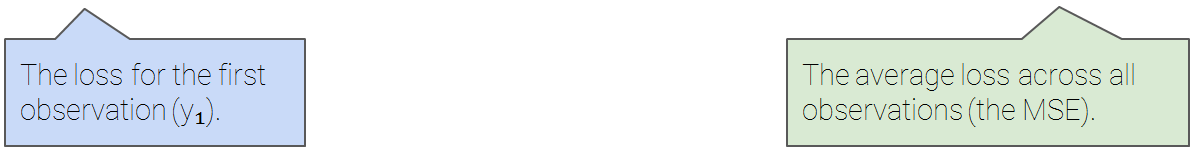
\includegraphics[scale=.4]{Bild25}
	\end{frame}
	
	
	
	\begin{frame}{Exploring MSE}
	        $L_2(20,\theta) = (20 - \theta)^2 \hspace{1cm} R(\theta) = \frac{1}{5}((20 - \theta)^2 + (21-\theta)^2 + (22 - \theta)^2 + (29 - \theta)^2 + (33 - \theta)^2)$
	    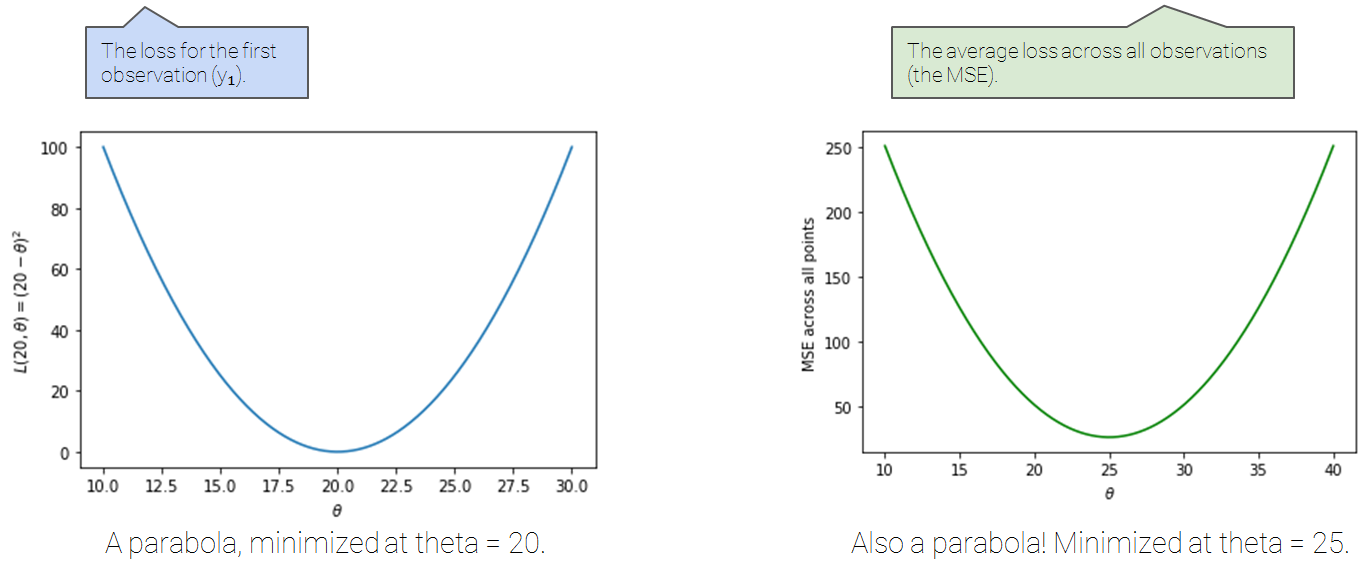
\includegraphics[scale=.4]{Bild26}
	\end{frame}
\end{document}